\documentclass{article}
\usepackage[utf8]{inputenc}
\usepackage{listings}
\usepackage{graphicx}
\usepackage{float}
\usepackage{xcolor}
\usepackage{geometry}
\usepackage{CJKutf8}
\usepackage{amsmath}
\usepackage{amssymb}

\geometry{a4paper,scale=0.8}
\lstset{
    basicstyle          =   \sffamily,        
    keywordstyle        =   \bfseries,         
    commentstyle        =   \rmfamily\itshape, 
    stringstyle         =   \ttfamily, 
    flexiblecolumns,               
    numbers             =   left,  
    showspaces          =   false, 
    showstringspaces    =   false,
    captionpos          =   t,     
    frame               =   lrtb, 
}

\lstdefinestyle{Python}{
    language        =   Python, % 语言选Python
    basicstyle      =   \zihao{-5}\ttfamily,
    numberstyle     =   \zihao{-5}\ttfamily,
    keywordstyle    =   \color{blue},
    keywordstyle    =   [2] \color{teal},
    stringstyle     =   \color{magenta},
    commentstyle    =   \color{red}\ttfamily,
    breaklines      =   true,  
    columns         =   fixed,  
    basewidth       =   0.5em,
}

\title{\bf\Large  概率论与数理统计 第13次作业}
%%%%%%%%%%%%%%%%%%%%%%%%%%%%%%%%%%%%%%
%% DON'T forget to change this part %%
\author{\bf Name: 宋昊原 \qquad Student ID: 2022010755}
%%%%%%%%%%%%%%%%%%%%%%%%%%%%%%%%%%%%%%

\begin{document}
\begin{CJK}{UTF8}{gbsn}
\maketitle
\section{对偶关系}
\subsection{单侧检验}
设
$$ H_{0}:\ \mu\leq\mu_{0} $$
$$ H_{1}:\ \mu>\mu_{0} $$
则拒绝域形状为
$$ \bar{X}>c $$
则
$$ {\rm P}_{\mu=\mu_{0}}(\bar{X}>c)=\alpha $$
由于
$$ \frac{\bar{X}-\mu}{S/\sqrt{n}}\sim{\rm t}(n-1)$$
当$\mu=\mu_{0}$时,上述概率为
$$ c = \mu_{0}+\frac{S}{\sqrt{n}}t_{\alpha}(n-1)$$
即拒绝域为
$$ \{\mathbf{X}\vert\bar{X}>\mu_{0}+\frac{S}{\sqrt{n}}t_{\alpha}(n-1)\}$$
\subsection{单侧区间估计}
即需找到一个区间
$$ [\bar{X}-c,\ +\infty) $$
使得
$$ {\rm P}(\bar{X}-\mu\leq c)=1-\alpha $$
由于
$$ \frac{\bar{X}-\mu}{S/\sqrt{n}}\sim{\rm t}(n-1) $$
只需
$$ c = \frac{S}{\sqrt{n}}t_{\alpha}(n-1)$$
即$1-\alpha$置信的单侧区间估计为
$$ [\bar{X}-\frac{S}{\sqrt{n}}t_{\alpha}(n-1),\ +\infty)$$
于是,$\mu_{0}$属于置信区间等价于
$$ \bar{X}\leq\mu_{0}+\frac{S}{\sqrt{n}}t_{\alpha}(n-1)$$
这等价于不拒绝$H_{0}$.
\section{元件寿命}
\subsection{}
取
$$ H_{0}:\ \mu\leq 225 $$
$$ H_{1}:\ \mu>225 $$
此时拒绝域为
$$ \bar{X}>225+\frac{S}{\sqrt{n}}t_{\alpha}(n-1)$$
计算得
$$ 225+\frac{S}{\sqrt{n}}t_{\alpha}(n-1)=268.3 $$
$$ \bar{X}=241.5 $$
故没有理由拒绝$H_{0}$,即没有理由认为元件平均寿命大于225小时.
\subsection{}
检验P值为
$$ {\rm P}_{\mu=225}(\bar{X}\geq 241.5)={\rm P}_{\mu=225}(\frac{\bar{X}-\mu}{S/\sqrt{n}}\geq 0.6685)=0.2570>0.05$$
\section{心脏病与胆固醇}
设无明显心脏病组胆固醇含量服从${\rm N}(\mu_{1},\sigma_{1}^{2})$,有明显心脏病组胆固醇含量服从${\rm N}(\mu_{2},\sigma_{2}^{2})$,取
$$ H_{0}:\ \mu_{1}=\mu_{2} $$
$$ H_{1}:\ \mu_{1}<\mu_{2} $$
由于近似地有
$$ \frac{(\bar{X_{1}}-\bar{X_{2}})-(\mu_{1}-\mu_{2})}{\sqrt{S_{1}^{2}/n_{1}+S_{2}^{2}/n_{2}}}\sim {\rm N}(0,1)$$
拒绝域为
$$ \bar{X_{1}}-\bar{X_{2}}<-\sqrt{\frac{S_{1}^{2}}{n_{1}}+\frac{S_{2}^{2}}{n_{2}}}Z_{\alpha} $$
计算得
$$ -\sqrt{\frac{S_{1}^{2}}{n_{1}}+\frac{S_{2}^{2}}{n_{2}}}Z_{\alpha}=-38.91 $$
$$ \bar{X_{1}}-\bar{X_{2}}=-20.92 $$
故不能认为两组胆固醇含量有显著差异.
\\\\
检验的P值为
$$ {\rm P}_{\mu_{1}=\mu_{2}}(\bar{X_{1}}-\bar{X_{2}}\leq =-20.92)=0.1055 $$
\section{假设检验判断题}
(1)(3)均错误,假设检验不可能得到完全确切的结果.
\\\\
(2)(4)均错误,哪个假设成立在进行检验前就已经确定,最后的决策只是根据样本情况对已经确定的假设成立情形的一个推测,不存在“假设为真的概率”.
\\\\
(5)错误,拒绝原假设时知道自己出错的概率仍然是在说“知道原假设为真的概率”,而这个概率没有意义.
\\\\
(6)错误,这里的P值的含义是,如果原假设为真,则大量重复这个实验,有99.9\%的可能性不会出现当前结果或比当前结果更极端的结果.\ 但由于原假设是否为真我们无法确知,所以仍然不能得出(6)的结论.
\section{Mendel\ 9:3:3:1}
$$ O_{1}=315,\ O_{2}=101,\ O_{3}=108,\ O_{4}=32 $$
$$ E_{1}=312.75\ E_{2}=104.25,\ E_{3}=104.25,\ E_{4}=34.75$$
于是
$$ \chi^{2}=\sum\limits_{i=1}^{4}\frac{(O_{i}-E_{i})^{2}}{E_{i}}=0.47 $$
计算得P值为0.9254,即几乎没有理由拒绝Mendel理论给出的概率分布.
\section{不同容量的卡方检验}
\subsection{}
卡方值为1,自由度5,P值0.9626.
\\\\
几乎没有理由拒绝骰子均匀.
\subsection{}
卡方值为10,自由度5,P值0.0752.
\\\\
如果选择较粗略的显著性水平(如$\alpha=0.1$)就已经可以拒绝骰子均匀的假设,或者说,可以不太显著地认为骰子不均匀.
\subsection{}
对给定的多项分布,样本容量越大,理论的相对误差就会越小.\ \ 如果一个大样本产生了像小样本一样的相对误差,则其P值会很低.
\section{吸烟有害健康}
观测频数:
$$ O_{11}=26,\ O_{12}=147,\ O_{13}=37 $$
$$ O_{21}=30,\ O_{22}=123,\ O_{23}=22 $$
计算期望频数:
$$ E_{11}=30.55,\ E_{12}=147.27,\ E_{13}=32.18 $$
$$ E_{21}=25.45,\ E_{22}=122.73,\ E_{23}=26.82 $$
则
$$ \chi^{2}=3.08 $$
自由度为
$$ (2-1)\times(3-1)=2 $$
故计算得P值为
$$ 0.2143 $$
这说明在$\alpha=0.1$显著性水平下,不能认为吸烟量与慢性支气管炎有显著相关性.
\section{伪造的杂交实验}
计算出$\chi^{2}=0.5103$,自由度为3,故P值为
$$ 0.9166 $$
这说明在Mendel遗传规律的前提下,有0.0834的可能性产生比此数据更“好”的数据,在$\alpha=0.05$的显著性水平下没有理由认为此数据是伪造的.
\section{计算机实验:假设检验}
\subsection{P值}
我进行了1000次检验并画出其P值分布,如下:\\
\begin{minipage}{0.5\textwidth}
    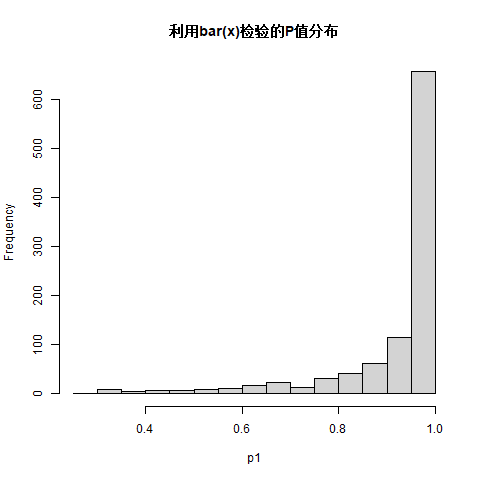
\includegraphics[scale=0.5]{check1.png}
\end{minipage}
\begin{minipage}{0.5\textwidth}
    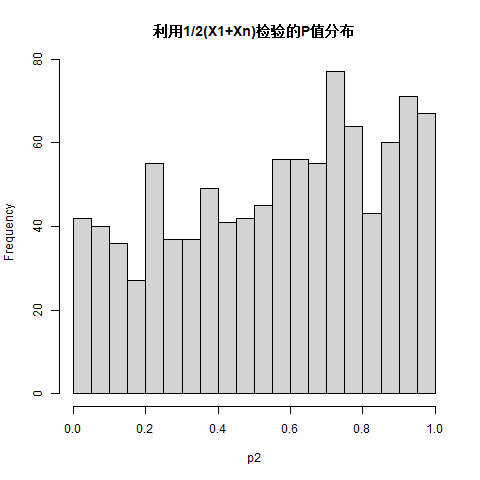
\includegraphics[scale=0.5]{check2.png}
\end{minipage}
\subsection{第一类错误}
反复进行实验,利用$\bar{X}$检验,第一类错误几乎不会发生,偶尔会在1000次内发生1次,与0.05的频率差别很大.\ \ 而利用$\frac{1}{2}(X_{1}+X_{n})$检验,第一类错误在1000次内发生的次数在30次上下,与0.05有一定差距但比较接近.
\\\\
这是因为真实的分布均值5本身已经与检验标准5.2有一定差距,因此会较难拒绝原假设,且检验使用的样本容量越大,拒绝原假设就会越难.
\end{CJK}
\end{document}